\chapter{Línguas de Sinais, Tecnologia e Educação: Um Mapeamento Sistemático}
\label{chapter:mapeamento-sistematico}

\section{Considerações iniciais}
\label{ms:inicio}

A adoção de TICs como ferramentas de TA para a educação inclusiva se mostra uma iniciativa promissora para a criação de soluções mais robustas e sensíveis ao contexto de PcD. Sendo assim, identificar estudos que relacionem esses conceitos, no âmbito das línguas de sinais, se demonstrou fundamental para a análise e elaboração de uma proposta de projeto coerente, tendo em vista o estado da prática a respeito do uso da tecnologia para o ensino e aprendizagem por meio das línguas de sinais.

Nesse contexto, as seções a seguir apresentam todo processo de condução de um MS, que buscou contribuições que relacionam os conceitos de línguas de sinais, tecnologia e educação, considerando questões de pesquisa pertinentes aos objetivos deste trabalho. A \autoref{ms:conducao} apresenta os detalhes sobre o protocolo, execução, extração de dados e resultados, já a \autoref{ms:sintese-resultados} discute os principais estudos primários sob as perspectivas internacional e nacional. Por fim, a \autoref{ms:fim} discorre brevemente sobre algumas considerações finais.

\section{Mapeamento Sistemático}
\label{ms:conducao}

Segundo \citeonline{Kitchenham2007}, existem duas abordagens principais para a condução de estudos sistemáticos de literatura. A primeira delas é a Revisão Sistemática (RS), definida como um estudo secundário que usa uma metodologia para identificar, analisar e interpretar todas as evidências relacionadas a uma questão de pesquisa com um escopo bem definido, de forma replicável e menos propensa a viés.

\citeonline{Kitchenham2007} também definem um segundo tipo de estudo, denominado Mapeamento Sistemático (MS), que tem como objetivo apresentar as evidências de um domínio de estudo em um alto nível de granularidade, agrupando as evidências encontradas em áreas de similaridade e geralmente identificando linhas de pesquisa em ascensão e/ou áreas com contribuições científicas escassas.

Adicionalmente, \citeonline{Petersen2015} mencionam que a técnica de MS é recomendada quando há a falta de estudos primários relevantes e de alta qualidade. O MS é recomendado, em detrimento de uma RS, quando o tópico for muito abrangente ou existam poucas evidências a serem coletadas em um domínio mais específico. Dessa forma, tendo em vista um escopo de pesquisa amplo (buscando a convergência entre três grandes áreas: tecnologia, educação e línguas de sinais), optou-se pela condução de um MS. 
%O MS conduzido buscou verificar o cenário atual de pesquisas envolvendo temáticas que relacionem os conceitos de ensino e aprendizagem por meio das línguas de sinais mediante o uso de tecnologia. 

Para isso, algumas das principais diretrizes disponíveis na literatura foram utilizadas no desenvolvimento deste estudo. Especificamente, as diretrizes de \citeonline{Kitchenham2007, Zhang2011, Petersen2015} foram consideradas na definição do protocolo de busca e processo de condução deste MS. Além disso, por meio da categorização, o MS pode fornecer um resumo visual e conciso sobre as temáticas/questões investigadas \cite{Petersen2008}.

Segundo \citeonline{Nakagawa2010}, o primeiro e mais importante passo para obter sucesso em um MS é planejá-lo corretamente. Desta forma, com base nas diretrizes citadas previamente, foi definido um protocolo que explorou estrategicamente cada uma das diretrizes \cite{Kitchenham2007,Zhang2011,Petersen2015}.

Nesse sentido, a abordagem proposta por \citeonline{Zhang2011} tem maior destaque neste MS, pois nossa estratégia de busca e critérios de qualidade se basearam nas diretrizes propostas pelos autores. A \autoref{ms:zhang-approach} sintetiza a abordagem de pesquisa sistemática em questão, a qual foi adaptada para este estudo, visando aumentar o rigor do processo de pesquisa por meio do \textit{Quasi-Gold Standard} (QGS) em conjunto com algumas das boas práticas propostas pelas diretrizes de \citeonline{Kitchenham2007} e \citeonline{Petersen2015}.

\begin{figure}[htbp]
\caption{Busca sistemática baseada em QGS.}
\label{ms:zhang-approach}
\centerline{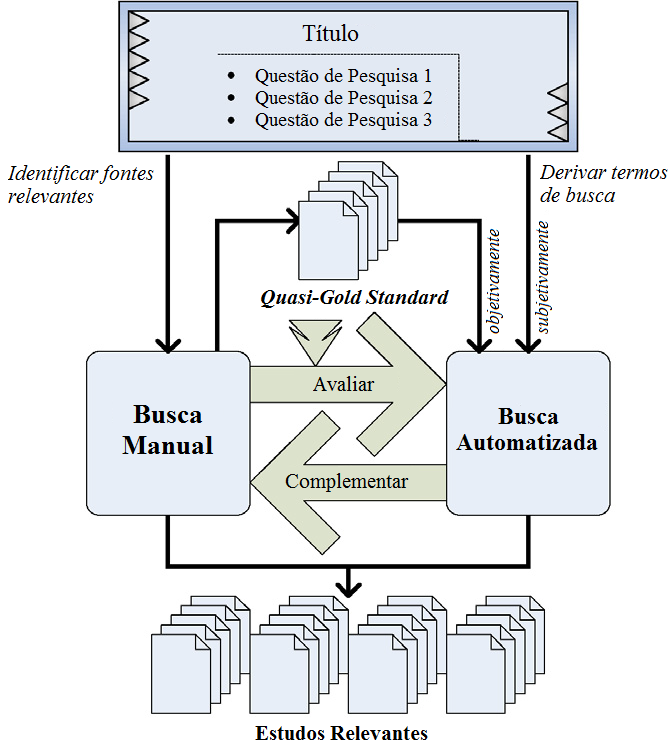
\includegraphics[width=0.55\textwidth]{images/zhang-systematic-mapping-approach.png}}
\caption*{Fonte: \citeonline{Zhang2011}.}
\end{figure}

Considerando a \autoref{ms:zhang-approach} é possível interpretar, em alto nível, a dinâmica da abordagem de \citeonline{Zhang2011}. Primeiramente, as questões de pesquisa devem ser definidas, juntamente com seus respectivos critérios de seleção\iffalse(Subseções \ref{ms:conducao-escopo} e \ref{ms:conducao-busca})\fi. Em seguida, as fontes para a busca manual\iffalse(\autoref{ms:conducao-busca-manual})\fi e os termos para a busca automatizada\iffalse(\autoref{ms:conducao-busca-automatizada})\fi são identificados/derivados. Com isso, o processo de busca manual define um conjunto de estudos primários relevantes, chamado de QGS. Através do QGS, a busca automatizada é avaliada e, se necessário, novas iterações podem ser realizadas (com o objetivo de refinar a busca automatizada) até que a qualidade seja considerada adequada pelo cálculo da \textit{quasi-sensitivity} (\autoref{ms:zhang-approach-steps})\iffalse, mais detalhes na Subseção \ref{ms:conducao-busca-performance}\fi. Por fim, os estudos selecionados pela busca automatizada, juntamente com o QGS (definido na busca manual), são classificados como relevantes/primários possibilitando a extração dos dados com o objetivo de responder às questões de pesquisa\iffalse(Subseções \ref{ms:conducao-extracao-dados} e \ref{ms:resultados})\fi.

\begin{figure}[htbp]
\caption{Etapas busca sistemática baseada em QGS.}
\label{ms:zhang-approach-steps}
\centerline{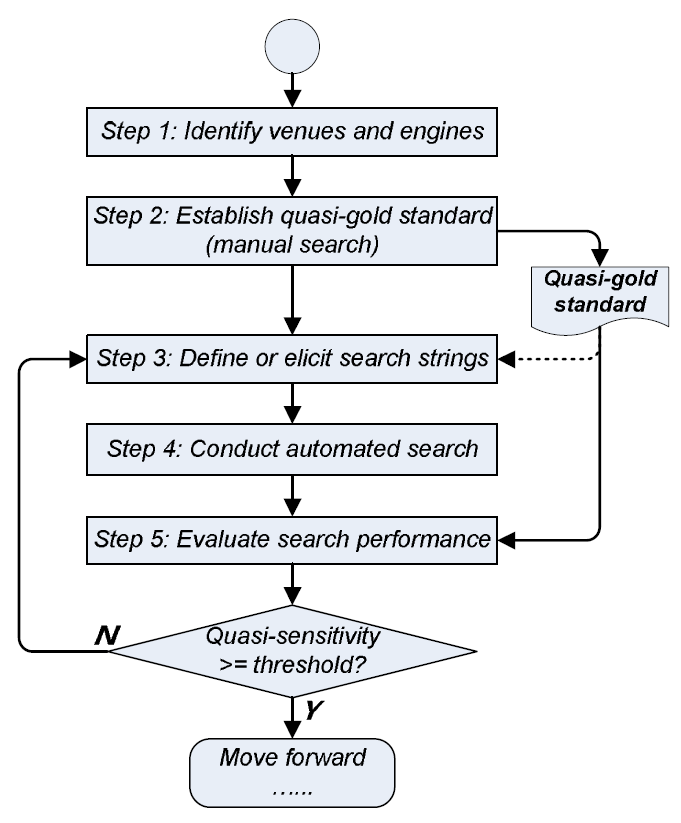
\includegraphics[width=0.625\textwidth]{images/zhang-systematic-mapping-steps.png}}
\caption*{Fonte: \citeonline{Zhang2011}.}
\end{figure}

\subsection{Definição do Escopo}
\label{ms:conducao-escopo}

As Questões de Pesquisa (QP) são essenciais para definir o escopo e identificar possíveis palavras-chave em um estudo sistemático de literatura \cite{Kitchenham2007,Petersen2015}. Neste contexto, uma abordagem comumente usada se dá através da aplicação dos critérios de PICO. Segundo \citeonline{Petticrew2008}, as QP podem ser estruturadas sob quatro aspectos: \textit{Population} (População); \textit{Intervention} (Intervenção); \textit{Comparison} (Comparação); e \textit{Outcome} (Resultados). Os critérios de PICO são apresentados na \autoref{table:pico}.

\begin{table}[!ht]
\caption{Critérios de PICO.}
\label{table:pico}
\centering
\begin{tabular}{ll}
\toprule
\textbf{\textit{Population}} & Alunos/Aprendizes de línguas de sinais. \\
\textbf{\textit{Intervention}} & Tecnologias relevantes para o ensino por meio das línguas de sinais. \\
\textbf{\textit{Comparison}} & Não se aplica. \\
\textbf{\textit{Outcome}} & Panorama tecnológico sobre o ensino baseado em línguas de sinais. \\ 
\bottomrule
\end{tabular}
\fautor
\end{table}

Por meio dos critérios definidos no PICO é possível identificar, de forma abstrata, o escopo do MS proposto. Sendo assim, o objetivo deste MS é determinar como a tecnologia está sendo aplicada no ensino e aprendizagem baseado em línguas de sinais, o que derivou as seguintes QP:

\begin{itemize}
    \item \textbf{QP1}: Quais aspectos de desenvolvimento estão sendo utilizados na construção de aplicações para o ensino e aprendizagem por meio das línguas de sinais?
    \begin{itemize}
        \item Quais são os tipos de soluções propostas (software ou hardware ou teóricas)?
        \item Quais tecnologias foram usadas?
        \item Quais métodos de avaliação foram aplicados?
    \end{itemize}
    \item \textbf{QP2}: Quais tópicos educacionais são abordados?
    \item \textbf{QP3}: Quais línguas de sinais são abordadas?
    \begin{itemize}
        \item Quais estudos abordam múltiplas línguas de sinais?
    \end{itemize}
\end{itemize}

De acordo com  \citeonline{Kitchenham2007}, um dos objetivos de um MS é realizar um levantamento de estudos relevantes para avaliar a quantidade de evidências existentes, visando responder as questões de pesquisa propostas. Segundo \citeonline{Felizardo2012}, o processo precisa ser rigoroso e imparcial, além de envolver uma ampla cobertura de fontes de informação, como bancos de dados, periódicos e conferências. Além disso, para minimizar o viés e maximizar o número de estudos examinados, é necessária uma estratégia de busca bem definida. %A seguir, apresentamos em mais detalhes nossa abordagem de pesquisa, juntamente com seus critérios de seleção e avaliação da qualidade.

\subsection{Critérios de Seleção}
\label{ms:conducao-busca}

Segundo \citeonline{Kitchenham2007,Petersen2015}, os estudos sistemáticos requerem critérios explícitos de inclusão e exclusão para avaliar seus potenciais estudos primários. Assim, foram definimos os seguintes critérios de seleção:

\begin{table}[htbp]
\caption{Critérios de Inclusão (CI) e Exclusão (CE)}
\label{tab:ms:criterios-selecao}
\begin{tabularx}{\textwidth}{C{1cm}|X} \hline
\textbf{CI1} & Os estudos apresentam contribuições (software ou hardware ou teóricas) para o ensino e a aprendizagem de línguas de sinais. \\ \hline
\textbf{CE1} & Estudos que não foram publicados no período de 2000 a 2019, seguindo um racional semelhante à \citeonline{Radermacher2013,Scatalon2019}, os quais sugerem que estudos anteriores a 2000 não representam as abordagens educacionais atuais, especialmente considerando o contexto de tecnologia. \\ \hline
\textbf{CE2} & Estudos classificados como resumos, resumos de conferências/editoriais, literatura cinza ou capítulos de livros. \\ \hline
\textbf{CE3} & Estudos não apresentados em inglês ou português. \\ \hline
\textbf{CE4} & Estudos não acessíveis em texto completo. \\ \hline
\textbf{CE5} & Estudos duplicados ou superficialmente complementares de outros estudos. \\ \hline
\end{tabularx}
\fautor
\end{table}

%\begin{itemize}
%    \item Critério de Inclusão:
%    \begin{itemize}
%        \item Os estudos apresentam contribuições (software ou hardware ou teóricas) para o ensino e a aprendizagem de línguas de sinais.
%    \end{itemize}
%    \item Critérios de Exclusão:
%    \begin{itemize}
%        \item Estudos que não foram publicados no período de 2000 a 2019, seguindo um racional semelhante à \citeonline{Radermacher2013,Scatalon2019}, os quais sugerem que estudos anteriores a 2000 não representam as abordagens educacionais atuais, especialmente considerando o contexto da ES;
%        \item Estudos que não estão no campo da ES;
%        \item Estudos classificados como resumos, resumos de conferências/editoriais, literatura cinza ou capítulos de livros;
%        \item Estudos não apresentados em inglês ou português;
%        \item Estudos não acessíveis em texto completo;
%        \item Estudos duplicados ou superficialmente complementares de outros estudos.
%    \end{itemize}
%\end{itemize}

Ainda sobre os critérios de exclusão, alguns esclarecimentos são pertinentes. Primeiro, o inglês e o português foram escolhidos porque o primeiro é o idioma mais indexado pelos mecanismos de busca e o segundo é o idioma nativo dos autores. Além disso, se pretende obter uma visão geral das contribuições em português. Por fim, foram classificados como ``estudos não acessível em texto completo'' os trabalhos não cobertos por acesso institucional. Com isso, estudos pagos e/ou inacessíveis, foram desconsiderados.

%A seguir, apresentamos nossa busca manual e seus respectivos estudos selecionados que, por definição, representariam nosso QGS. Entretanto, a \autoref{ms:conducao-busca-manual} discorre sobre decisões importantes com relação à composição do QGS, pautadas principalmente pela grande diferença na qualidade de indexação entre as fontes nacionais e internacionais. Com isso, nosso QGS foi composto majoritariamente por estudos selecionados internacionalmente. Assim, a coesão entre a nossa estratégia de busca manual e a abordagem de \citeonline{Zhang2011} se mostrou mais adequada.

\subsection{Busca Manual}
\label{ms:conducao-busca-manual}

Para a etapa de busca manual, foram selecionadas fontes (periódicos e conferências) com ênfase em tecnologia e educação. %As fontes nacionais e internacionais foram definidas com o apoio de especialistas em ES do LabES\footnote{Laboratório de Engenharia de Software do ICMC--USP}. 
Nesta etapa, o conjunto \textit{title-abstract-keywords} foi utilizado para a avaliação dos estudos. De modo adicional, eventualmente outras seções foram lidas, visando uma classificação mais assertiva com base nos critérios de seleção propostos.

A \autoref{ms:table:busca-manual-nacional} apresenta as conferências e periódicos nacionais considerados durante a busca manual. Entretanto, os estudos obtidos dessas fontes foram desconsiderados na composição do QGS, pois a maioria das conferências/periódicos brasileiros não são indexados pelos mecanismos de busca internacionais e isso reduziria consideravelmente a eficácia da abordagem de busca sistemática baseada em QGS \cite{Zhang2011}. Todavia, os 46 estudos primários selecionados em fontes brasileiras foram devidamente considerados e discutidos nos resultados deste MS. 

\begin{table}[htbp]
\centering
\caption{Busca manual nacional}
\label{ms:table:busca-manual-nacional}
\begin{tabular}{lcc}
\hline
\textbf{Conferências/Periódicos} & \textbf{Fonte} & \textbf{Selecionados} \\ \hline
DesafIE                          & CEIE           & -                     \\
JAIE                             & CEIE           & -                     \\
RBIE                             & CEIE           & 2                     \\
RENOTE                           & CINTED         & 13                    \\
SBIE                             & CEIE           & 13                    \\
WAVE2                            & CEIE           & -                     \\
WCBIE                            & CEIE           & 11                    \\
WIE                              & CEIE           & 7                     \\
\multicolumn{2}{l}{\textbf{Total}}                & \textbf{46}           \\ \hline
\end{tabular}
\fautor
\end{table}

A \autoref{ms:table:busca-manual-internacional} apresenta as conferências e periódicos internacionais considerados durante a busca manual. Essa etapa resultou na seleção de 19 estudos primários, que representam o QGS deste MS. Considerando as Bibliotecas/Editoras em questão, todas as fontes relevantes (com ao menos um estudo selecionado) podem ser obtidas pelas seguintes fontes: ACM (ACM Digital Library), IEEE (IEEE Xplore), Elsevier (ScienceDirect) e Springer (Springer Link). De acordo com \citeonline{Zhang2011}, é apropriado que essas mesmas bases de dados sejam utilizadas para executar a busca automatizada, gerando assim uma sinergia maior com o QGS.

\begin{table}[htbp]
\centering
\caption{Busca manual internacional (QGS)}
\label{ms:table:busca-manual-internacional}
\begin{tabular}{lcc}
\hline
\textbf{Conferência/Periódico} & \textbf{Fonte}     & \textbf{Selecionados (QGS)} \\ \hline
ACM TOCE                       & ACM                & 0            \\ 
Computers \& Education         & Elsevier           & 5            \\ 
FIE                            & IEEE               & 0            \\ 
HCI International              & Springer           & 5            \\ 
ICALT                          & IEEE               & 5            \\ 
IEEE Trans. Educ.              & IEEE               & 1            \\ 
IEEE Trans. Learn. Technol.    & IEEE               & 0            \\ 
Informatics in Education       & Vilnius University & 0            \\ 
ITiCSE                         & ACM                & 2            \\ 
Learning @ Scale               & ACM                & 0            \\ 
SIGCSE                         & ACM                & 1            \\ 
\textbf{Total}                 & \textbf{}          & \textbf{19}  \\ \hline
\end{tabular}
\fautor
\end{table}

Por fim, em atenção à abordagem de busca sistemática baseada em QGS, se faz necessário esclarecer algumas definições. Primeiramente, o termo \textit{Gold Standard} representa todos os estudos primários possíveis de uma questão de pesquisa, ou seja, algo difícil de se obter. Por outro lado, o QGS representa um subconjunto desses estudos, tornando-se uma alternativa mais viável \cite{Zhang2011}. Portanto, \citeonline{Zhang2011} sugerem a criação do QGS a partir dos estudos selecionados pela busca manual (\autoref{ms:table:busca-manual-internacional}), com o objetivo de aferir a qualidade da busca automatizada. Para isso, a \textit{quasi-sensitivity} foi utilizada, uma fórmula que avalia o desempenho dessa busca, que idealmente deve incluir a maior parte dos estudos do QGS. 

A seguir é descrita a busca automatizada conduzida, tendo em vista as bases de dados e estudos relevantes (QGS) identificados mediante o processo de busca manual supracitado. Além disso, o processo de avaliação de performance da busca automatizada por meio da \textit{quasi-sensitivity} é devidamente detalhado.

\subsection{Busca Automatizada}
\label{ms:conducao-busca-automatizada}

Antes de realizar uma busca automatizada, é essencial definir os critérios para criação de uma string de busca. Nesse sentido, duas estratégias para identificação de palavras-chave foram utilizadas em conjunto: (i) análise do PICO e suas respectivas QP; (ii) importação da tripla \textit{title-abstract-keywords} em um software de análise de frequência. Os resultados desse processo produziram a seguinte string de busca:

\begin{center}
    (\textit{learn} \textbf{OR} \textit{learning} \textbf{OR} \textit{teach} \textbf{OR} \textit{teaching}) \textbf{AND}\\
    (``\textit{sign language}'' \textbf{OR} ``\textit{signed language}'') \textbf{AND}\\
    (\textit{technology} \textbf{OR} \textit{technologies})\\
\end{center}

Seguindo a proposta de \citeonline{Zhang2011}, foi realizada a busca automatizada nas quatro bases de dados identificadas como relevantes pela busca manual: ACM Digital Library\footnote{https://dl.acm.org}, IEEE Xplore\footnote{https://ieeexplore.ieee.org}, ScienceDirect\footnote{https://sciencedirect.com}, Springer Link\footnote{https://link.springer.com}. %Portanto, a string de busca em questão foi executada nessas máquinas de busca.
A \autoref{method:table:automated-search} resume os resultados da busca automatizada, onde a seleção dos estudos seguiu o mesmo racional apresentado na busca manual. Além disso, a busca automatizada retornou a maioria dos estudos selecionados pela busca manual (QGS), o que sugere uma boa sensibilidade da string de busca. %Nesse sentido, mais detalhes são discutidos na seção a seguir.

\begin{table}[htbp]
\centering
\caption{Resultados da busca automatizada}
\label{method:table:automated-search}
\begin{tabular}{lllll}
\hline
 &  & Busca Final &                 &                   \\ \cline{3-5} 
Base de Dados & \textbf{QGS} & Recuperados    & \textbf{no QGS} & \textbf{Relevantes} \\ \hline
ACM DigitalLibrary & 3            & 922          & 3               & 47                \\
IEEE Xplore        & 6            & 359          & 5               & 59                \\
ScienceDirect      & 5            & 1,961        & 5               & 20                \\
SpringerLink       & 5            & 4,980        & 5               & 36                \\
\textbf{Total}   & \textbf{19}  & 8,222        & \textbf{18}     & \textbf{162}      \\ \hline
\end{tabular}
\fautor
\end{table}

\noindent
\textbf{Avaliação de Performance da Busca Automatizada}

Segundo \citeonline{Zhang2011}, a qualidade da busca automatizada de uma pesquisa cientifica pode ser avaliada usando critérios consolidados na literatura, como a sensibilidade e a precisão. Nesse sentido, os autores propõem o conceito de \textit{quasi-sensibilidade}, uma derivação da sensibilidade tradicional que incorpora o QGS como critério de qualidade (\autoref{method:equation:quasi-sensitivity}).

\begin{equation}
\label{method:equation:quasi-sensitivity}
\text{\textit{quasi-sensibility}} = \frac{\text{\textit{Estudos relevantes recuperados (\textbf{no QGS})}}}{\text{\textit{Total de estudos relevantes (\textbf{QGS})}}}
\end{equation}

Portanto, para avaliar o desempenho da busca automatizada, a \textit{quasi-sensitivity} foi calculada considerando os dados da \autoref{method:table:automated-search}. De acordo com \citeonline{Zhang2011}, quando o desempenho da pesquisa é aceitável (quase sensibilidade $\geq$ 80\%), os resultados da busca automatizada podem ser mesclados com o QGS e o processo de busca é finalizado (\autoref{ms:zhang-approach-steps}).

Como resultado, a \textit{quasi-sensitivity} foi calculada em 94,74\% (18/19), ou seja, o desempenho da pesquisa é aceitável \cite{Zhang2011}. Portanto, os 163 artigos selecionados pelas buscas manual e automatizada são potenciais estudos primários, devendo ser lidos na íntegra. Nesta etapa, 24 estudos foram excluídos de acordo com os critérios de inclusão e exclusão pré-estabelecidos. A \autoref{method:figure:evaluation-refinement} organiza os 139 estudos primários, tendo em vista a abordagem de busca sistemática baseada em QGS.

\begin{figure}[htbp]
\caption{Resultados da busca sistemática baseada em QGS.}
\label{method:figure:evaluation-refinement}
\centerline{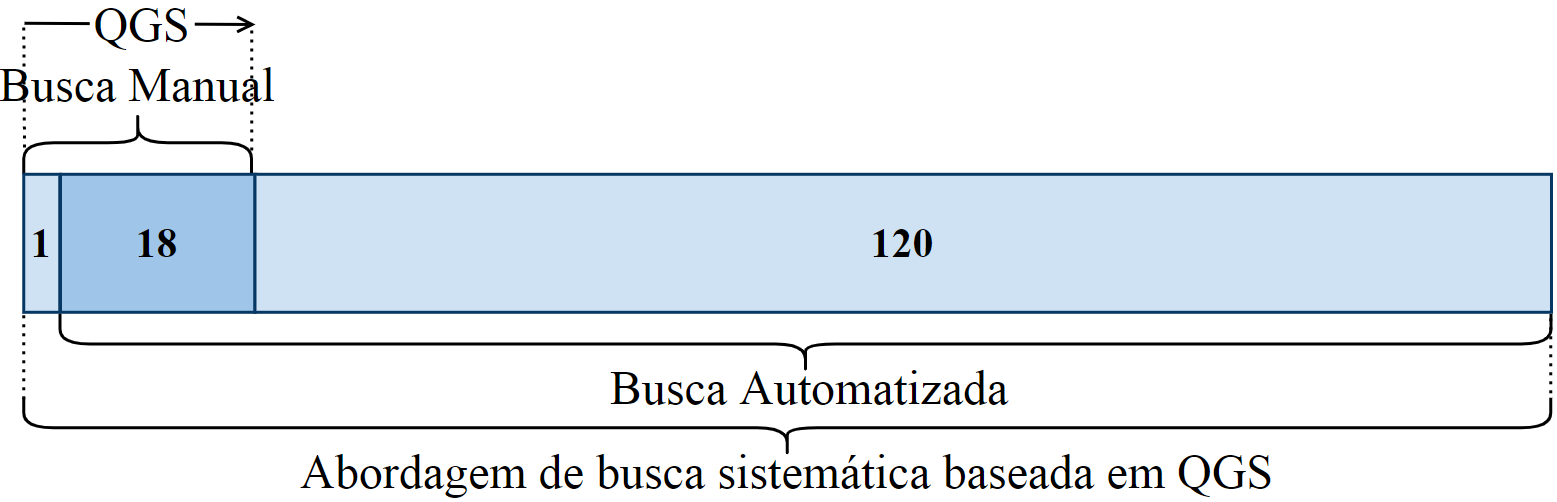
\includegraphics[width=0.8\textwidth]{images/systematic-mapping.png}}
\fautor
\end{figure}

\subsection{Extração de Dados}
\label{ms:conducao-extracao-dados}

Para extrair as informações relevantes dos estudos primários identificados, um formulário de extração de dados foi criado. O modelo na \autoref{method:table:data-extraction} descreve as informações extraídas e apresenta seu relacionamento com cada QP, quando aplicável.

\begin{table}[htbp]
\centering
\caption{Formulário de extração de dados}
\label{method:table:data-extraction}
\begin{tabular}{lll}
\hline
\textbf{Item} & \textbf{Descrição} & \textbf{QP} \\ \hline
\textit{\textbf{Informações Gerais}} & & \\ \hline
ID & Identificador (prefixos \textit{INT} ou \textit{BRA}). & \\
Título & Título do estudo. & \\
Autores & Nomes dos autores. & \\
Ano & Ano de publicação do artigo. & \\
Conferência/Periódico & Nome do meio de publicação. & \\
Tipo de busca & Manual; Automatizada; Ambas. & \\
Língua & Inglês; Português. & \\
País & País da afiliação do primeiro autor. & \\ \hline
\textit{\textbf{Informações Específicas}} & & \\ \hline
Área da ES & Área de conhecimento da ES (SWEBOK). & QP1 \\
Tipo de solução & Software; Hardware; Teórica. & QP1 \\
Estratégia empírica & Quais estratégias empíricas foram encontradas. & QP1 \\
Tópico educacional & Quais tópicos educacionais foram encontrados. & QP2 \\
Línguas de sinais & Quais línguas de sinais foram encontradas. & QP3 \\ \hline
\end{tabular}
\fautor
\end{table}

Devido ao grande número de estudos primários selecionados no MS, optou-se por não incluir todas as referências explicitamente neste trabalho. Sendo assim, todos os artigos e seus respectivos dados (incluindo um glossário para o formulário de extração de dados) estão disponíveis online\footnote{\url{https://bit.ly/SM-DataExtraction}}.

Os estudos primários oriundos de eventos \textit{Internacionais} (139 publicações selecionados por meio da abordagem de busca sistemática baseada em QGS); e \textit{Brasileiros} (46 publicações selecionadas por meio da busca manual nacional), foram devidamente identificados pelos prefixos \textit{INT} e \textit{BRA}. Assim, um total de 185 estudos primários foram identificados pelo MS, os quais são apresentados e discutidos nas seções a seguir.

\subsection{Resultados}
\label{ms:resultados}

Considerando os 185 estudos primários selecionados pelo MS, as informações mais relevantes para as QP foram sintetizadas seguindo a estrutura do formulário de extração de dados. Assim, nesta seção cada questão de pesquisa é abordada individualmente, evidenciando suas respectivas constatações. Antes disso, com base na análise de informações essenciais dos estudos, alguns cenários adicionais interessantes foram identificados. Com isso, foi possível estender os resultados deste MS por meio de informações transcendem as QP apresentadas.

Primeiramente, considerando a quantidade de publicações por ano, uma linha de tendência linear crescente foi identificada (\autoref{results:figure:publications-year}). Portanto, é estatisticamente possível que este domínio de pesquisa esteja em ascensão globalmente. Além disso, o número reduzido de publicações anteriores a 2010 (menos de 16\%) pode ser considerado para a definição de critérios de exclusão mais rigorosos em uma replicação ou atualização deste MS.

\begin{figure}[htbp]
\caption{Linha de tendência linear ($R^2$) de publicações internacionais por ano}
\label{results:figure:publications-year}
\centerline{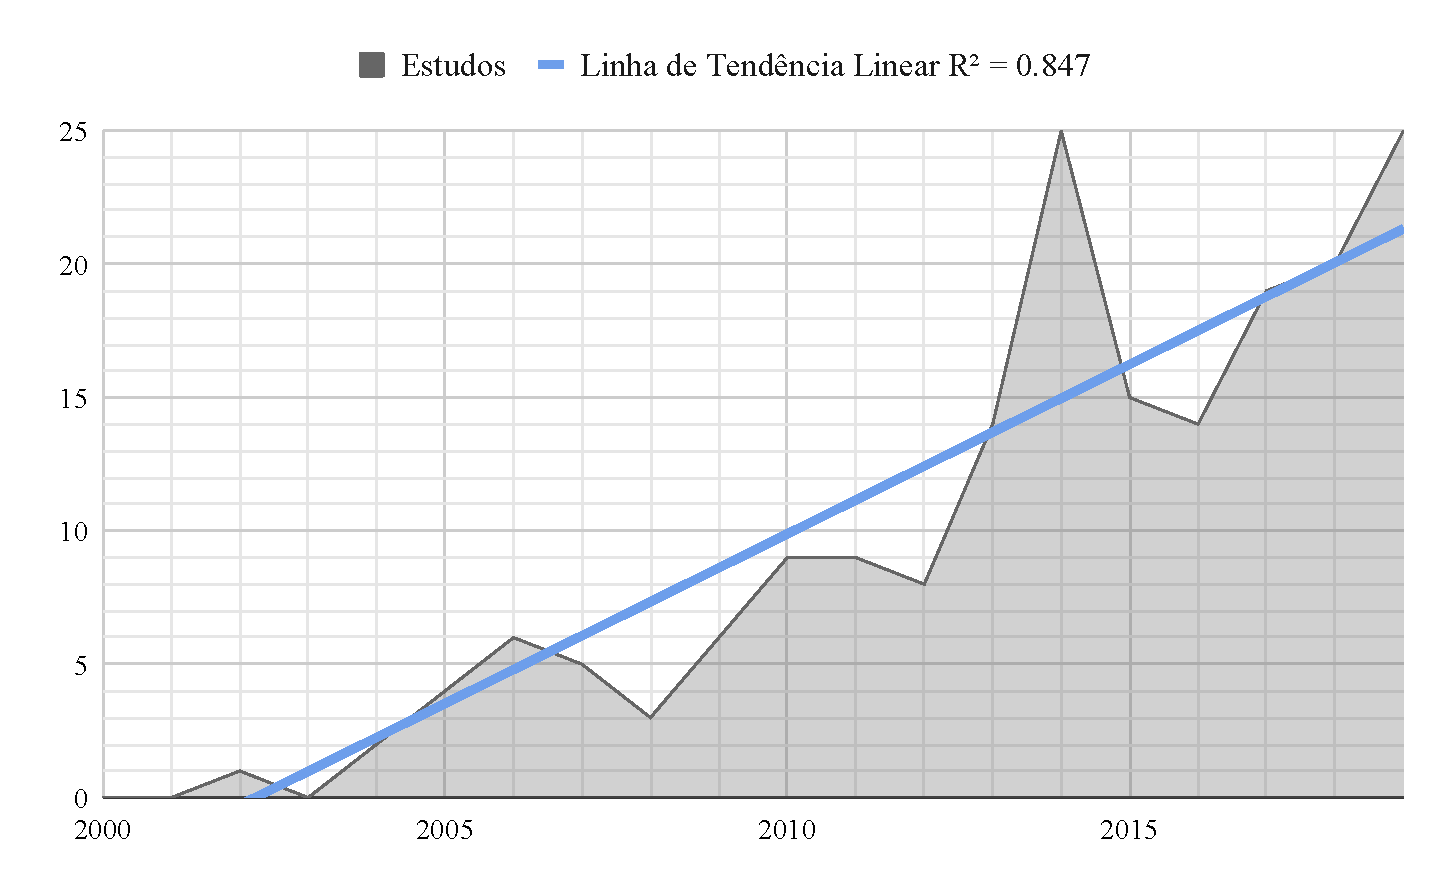
\includegraphics[width=\columnwidth]{images/publications-sm-timeline.pdf}}
\fautor
\end{figure}

%Outro dado relevante diz respeito às fontes das publicações, que também podem compor o racional das buscas manuais em possíveis estudos futuros. No contexto brasileiro, os 46 artigos classificados como relevantes na busca manual nacional podem ser avaliados sob essa perspectiva. Sendo assim, a Tabela \ref{results:table:manual-search-brazil} apresenta as conferências e periódicos destes estudos, que não foram considerados em nosso QGS porque as bases de dados, utilizadas nas buscas automatizadas, indexam predominantemente estudos em inglês. Considerando estes trabalhos, tem-se uma percepção mais assertiva com relação a Libras, tema onipresente nas publicações em questão.

%Por outro lado, a Tabela \ref{results:table:publication-venues} apresenta os principais locais de publicação, considerando os 139 estudos primários obtidos de fontes internacionais, os quais estão ordenados pela quantidade de estudos selecionados. Nesse contexto, a presença de conferências e periódicos definidos na busca manual internacional (em destaque na Tabela) sugere uma execução efetiva dessa fase considerando o protocolo de busca adotado.

Outro dado relevante diz respeito às fontes das publicações, que também podem compor o racional das buscas manuais em possíveis estudos futuros. A \autoref{results:table:publication-venues} apresenta os principais locais de publicação, considerando todos os estudos primários deste MS, os quais estão ordenados pela quantidade de estudos selecionados. No contexto internacional, a presença de conferências e periódicos definidos na busca manual (em destaque na tabela) sugere uma execução efetiva dessa fase considerando o protocolo de busca adotado.

\begin{table}[htbp]
\caption{Conferências/Periódicos mais relevantes}
\label{results:table:publication-venues}
\centering
\begin{tabular}{lcc|lcc}
\hline
\multicolumn{3}{c|}{\textbf{Internacionais (\textit{INT})}} & \multicolumn{3}{c}{\textbf{Nacionais (\textit{BRA})}} \\ \hline
\textbf{Nome} & \textbf{Fonte} & \textbf{Estudos} & \textbf{Nome} & \textbf{Fonte} & \textbf{Estudos} \\ \hline
\textit{\textbf{HCI International}} & \textit{\textbf{Springer}} & \textit{\textbf{12}} & RENOTE & CINTED & 13 \\ 
ICCHP & Springer & 8 & SBIE & CEIE & 13 \\ 
\textit{\textbf{ICALT}} & \textit{\textbf{IEEE}} & \textit{\textbf{6}} & WCBIE & CEIE & 11 \\ 
ASSETS & ACM & 6 & WIE & CEIE & 7 \\ 
\textit{\textbf{Computers \& Education}} & \textit{\textbf{Elsevier}} & \textit{\textbf{5}} & RBIE & CEIE & 2 \\ 
Procedia Computer Science & Elsevier & 5 & - & - & - \\ 
Outros & - & 97 & - & - & - \\ 
\multicolumn{2}{l}{\textbf{Total}} & \textbf{139} & \multicolumn{2}{l}{\textbf{Total}} & \textbf{46} \\ \hline
\end{tabular}
\fautor
\end{table}

Além disso, foi analisada a distribuição dos estudos primários internacionais por país de origem. Nesse contexto, identificou-se uma grande quantidade de publicações relevantes nos Estados Unidos e Brasil, com 22 e 21 artigos respectivamente, que juntos representam 31\% dos estudos primários deste MS. Com isso, mesmo desconsiderando os estudos selecionados pela busca manual nas fontes nacionais, o Brasil destacou-se internacionalmente na publicação de trabalhos que investigam o uso da tecnologia para o ensino e aprendizagem por meio das línguas de sinais.

%Lembrando que as conferências e periódicos das buscas manuais foram definidos com o apoio de especialistas nas áreas de ES e educação. Para isso, critérios como relevância do evento e facilidade no acesso às publicações foram levados em consideração. Entretanto, tais critérios são subjetivos e, portanto, estão sujeitos a viés. Além disso, alguns dos locais sugeridos (internacional e nacionalmente) não identificaram nenhum estudo relevante. Portanto, possíveis replicações deste MS devem ponderar eventuais evoluções nos eventos definidos para as buscas manuais.

A seguir são discutidos os principais resultados deste trabalho, de modo a responder cada QP definida no escopo do MS. Adicionalmente, com o objetivo de organizar os estudos primários, eles foram classificados com relação à sua origem: Internacional (\textit{INT})\footnote{Formulário de extração de dados --  INT: \url{https://bit.ly/SM-DataExtraction-INT}} ou Nacional (\textit{BRA})\footnote{Formulário de extração de dados --  BRA: \url{https://bit.ly/SM-DataExtraction-BRA}}. Com isso, os resultados podem ser isolados, o que pode beneficiar o planejamento e condução de trabalhos futuros.

\noindent
\textbf{Soluções Tecnológicas (QP1)}

%A primeira questão de pesquisa tem como objetivo identificar os tópicos formais da ES que também vêm sendo investigados e adotados no cenário da educação por meio das línguas de sinais. As áreas identificadas foram classificadas com base na estrutura \textit{Software Engineering Body of Knowledge} (\textit{SWEBOK}) \cite{Bourque2014, Petersen2015}.

A primeira questão de pesquisa têm como objetivo identificar as vertentes de desenvolvimento exploradas para a construção de soluções educacionais com apoio às línguas de sinais. Sendo assim, tendo em vista o aspecto multidisciplinar do desenvolvimento de software, optou-se pela classificação em áreas de conhecimento da ES. Para isso, as contribuições deste MS foram classificadas com base na estrutura \textit{Software Engineering Body of Knowledge} (\textit{SWEBOK}) \cite{Bourque2014, Petersen2015}.

Sendo assim, foram consideradas as quinze áreas possíveis da ES do \textit{SWEBOK}, das quais quatro foram investigadas pelos estudos primários deste MS. Essa concentração já era esperada, pois foi definido como objetivo identificar aspectos de desenvolvimento em um domínio específico, o que geralmente remete a áreas mais técnicas. A \autoref{results:table:se-areas} apresenta as áreas da ES identificadas nesta pesquisa, considerando os 185 estudos primários (139 Internacionais e 46 Brasileiros).

\begin{table}[htbp]
\caption{Áreas da ES (SWEBOK)}
\label{results:table:se-areas}
\centering
\begin{tabular}{lcccc}
\hline
                          & \multicolumn{2}{c}{\textbf{\textit{INT}}} & \multicolumn{2}{c}{\textbf{\textit{BRA}}} \\ \cline{2-5} 
\textbf{Área da ES}       & \textbf{Estudos} & \textbf{\%}             & \textbf{Estudos} & \textbf{\%}             \\ \hline
Construção de Software    & 65               & 47\%                    & 23               & 50\%                    \\ 
Projeto de Software       & 47               & 34\%                    & 5                & 11\%                    \\ 
Fundamentos da Engenharia & 24               & 17\%                    & 9                & 19\%                    \\ 
Qualidade de Software     & 3                & 2\%                     & 9                & 19\%                    \\ 
\textbf{Total}            & \textbf{139}     & \textbf{100\%} & \textbf{46}      & \textbf{100\%} \\ \hline
\end{tabular}
\fautor
\end{table}

\begin{itemize}
    \item \textbf{Construção de Software}: estudos com ênfase no desenvolvimento de soluções, incluindo seus respectivos detalhes de construção. Além disso, podem apresentar definições secundárias de \textit{design} e qualidade. Ainda, o projeto e implementação de APIs (\textit{Application Programming Interfaces}) também são classificados nessa área;
    \item \textbf{Projeto de Software}: estudos que apresentam conceitos de análise e projeto aplicados a soluções tecnológicas. Abstrações como arquiteturas e \textit{frameworks} também são comuns nessa vertente;
    \item \textbf{Fundamentos da Engenharia}: estudos com foco na avaliação empírica de suas soluções. Sendo assim, essa área possui relação direta com estudos de caso, \textit{surveys} e experimentos.
    \item \textbf{Qualidade de Software}: estudos com avaliações e validações não formais, relacionadas a critérios de qualidade minimamente estruturados. Revisões e auditorias de garantia de qualidade também são conduzidas nessa área.
\end{itemize}

Considerando as áreas da ES, é evidente que a maioria dos estudos primários apresentem o ``Projeto'' e ``Construção'' de soluções para o ensino/aprendizagem por meio das línguas de sinais. Por outro lado, existe uma quantidade importante de estudos com ênfase em avaliações empíricas, o que mostra a importância das avaliações formais na ES. Esses estudos foram classificados na área ``Fundamentos da Engenharia'' (\textit{INT8, INT9, INT11, INT12, INT17, INT22, INT30, INT31, INT32, INT33, INT38, INT39, INT40, INT43, INT45, INT77, INT83, INT84, INT91, INT93, INT98, INT113, INT130, INT131, BRA14, BRA17, BRA22, BRA27, BRA28, BRA35, BRA37, BRA40, BRA46}).

É importante observar, ainda, que muitos outros artigos apresentavam avaliações empíricas, mas foram classificados em outras áreas da ES, semanticamente mais adequadas a suas respectivas contribuições primárias. Nesse cenário, 47.5\% dos estudos primários do MS apresentaram algum tipo de avaliação empírica -- \textit{survey}, estudo de caso ou experimento \cite{Wohlin2012}. Por outro lado, considerando a busca manual nacional, essa porcentagem foi ligeiramente superior, com um total de 52.1\%. Assim, é possível aferir que aproximadamente a metade dos estudos primários identificados possuem algum tipo de avaliação formal.

No entanto, existe um número inferior de estudos com ênfase em avaliações não empíricas, cujo principal objetivo geralmente é conduzir validações menos estruturadas em um determinado domínio de aplicação. Tais estudos foram classificados como ``Qualidade de Software''. Nesse sentido, o MS retornou um número baixo de estudos com esta contribuição primária, cerca de 2\% (\textit{INT59, INT76, INT117}). Já a busca manual nacional obteve aproximadamente 19\% de seus estudos nesta categoria (\textit{BRA6, BRA7, BRA8, BRA9, BRA10, BRA11, BRA16, BRA18, BRA26}).%, evidenciando que esta é uma área da ES muito investigada no Brasil. 

De modo geral, as contribuições dos estudos primários foram classificadas em software, hardware ou teórica. Com isso, este trabalho identificou que 69.8\% de seus estudos têm ênfase em software, 11.3\% em hardware (\textit{INT11, INT12, INT19, INT43, INT58, INT61, INT65, INT67, INT71, INT88, INT97, INT102, INT105, INT108, INT125, INT133, INT137, INT138, BRA1, BRA14, BRA26}) e 18.9\% são contribuições teóricas (\textit{INT2, INT32, INT37, INT39, INT44, INT57, INT59, INT60, INT63, INT79, INT80, INT84, INT85, INT91, INT95, INT103, INT131, INT134, INT135, BRA6, BRA7, BRA8, BRA9, BRA10, BRA11, BRA13, BRA16, BRA17, BRA18, BRA22, BRA27, BRA28, BRA35, BRA37, BRA38}).

Desta forma, é possível concluir que a maioria das soluções tecnológicas para ensino e aprendizagem por meio de línguas de sinais vêm se baseando em software. Na \autoref{results:figure:publications-solutions} os estudos foram categorizados por seus respectivos tipos de solução. De acordo com a figura, observa-se a dominância de algumas plataformas de desenvolvimento de software: Web, Mobile e \textit{Desktop}. Juntas, essas plataformas equivalem a 52\% dos estudos primários. Também foram identificadas duas soluções que são claramente multiplataforma (\textit{INT70, INT116}). Essa pequena fração de contribuições pode denotar uma lacuna relevante em termos de usabilidade, já que a falta de uma experiência unificada pode prejudicar e/ou limitar a experiência dos usuários.

\begin{figure}[htbp]
\caption{Publicações por tipo de solução}
\label{results:figure:publications-solutions}
\centerline{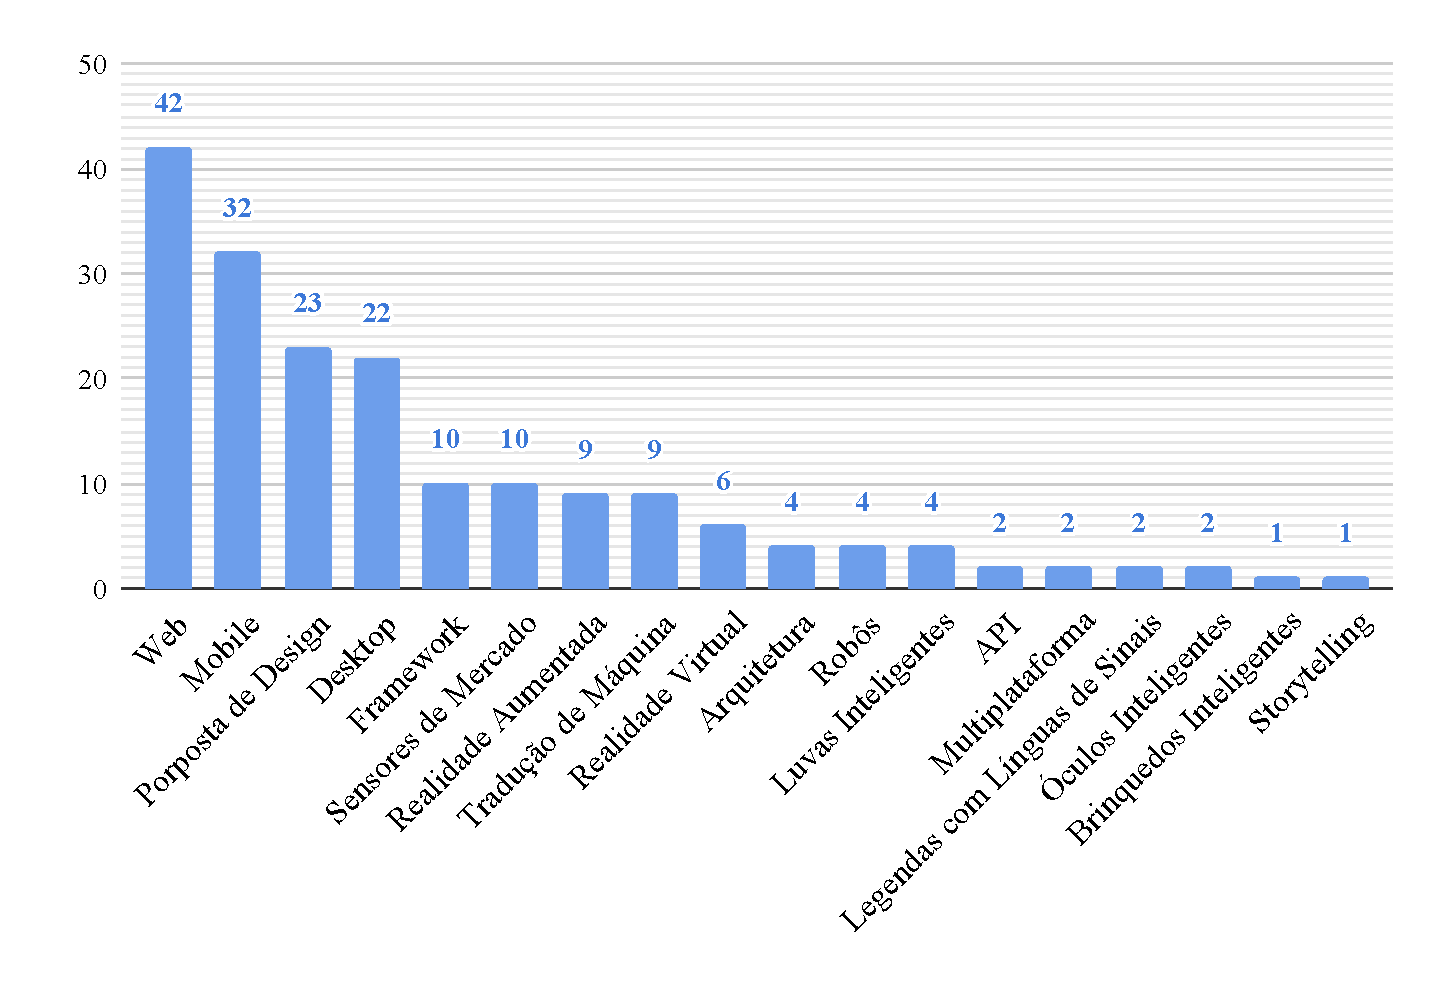
\includegraphics[width=\columnwidth]{images/publications-solutions.pdf}}
\fautor
\end{figure}

Sob outra perspectiva, diversas propostas de \textit{design} foram identificadas (\textit{INT2, INT26, INT27, INT32, INT38, INT39, INT40, INT44, INT79, INT80, INT84, INT85, INT87, INT95, INT130, INT131, INT134, BRA13, BRA17, BRA30, BRA32, BRA37, BRA38}), mostrando que os potenciais projetos vêm sendo avaliados pela comunidade científica antes de sua efetiva implementação.

Propostas relacionadas à tradução de máquina e legendas de línguas de sinais foram classificadas individualmente (\textit{INT5, INT10, INT17, INT20, INT21, INT47, INT54, INT82, INT86, INT121, INT129}). Com isso, foi possível obter uma visão mais técnica sobre a complexidade e os desafios encontrados nesse tipo de solução, geralmente investigadas por meio de abordagens de Inteligência Artificial (IA). Nessas vertentes, não foram identificados artigos na busca manual nacional, porém três publicações do MS aplicam tais técnicas no contexto da Libras (\textit{INT17, INT20, INT47}). 

Uma quantidade significativa de estudos têm ênfase em sensores de mercado (\textit{INT19, INT43, INT58, INT61, INT97, INT105, INT108, INT138, INT123, BRA1}), sendo os sensores Kinect\footnote{https://developer.microsoft.com/pt-br/windows/kinect}, Leap Motion\footnote{https://developer.leapmotion.com} e Myo Armband\footnote{https://developerblog.myo.com} os mais utilizados, nesta ordem. Isso evidencia que existem iniciativas na indústria que viabilizam o desenvolvimento de soluções para o reconhecimento de línguas de sinais por meio de hardware padronizados, comumente munidos de um Kit de Desenvolvimento de Software (SDK -- \textit{Software Development Kit}).

Por fim, os estudos primários demonstram que algumas técnicas e tecnologias vêm ganhando notoriedade. Nesse sentido, merece destaque o uso dos conceitos de Realidade Aumentada (RA) e Realidade Virtual (RV) em diversas soluções (\textit{INT34, INT46, INT69, INT77, INT96, INT106, INT124, INT135, BRA25, BRA29, BRA31}). Além disso, algumas API, \textit{frameworks} e arquiteturas de software foram propostas (\textit{INT49, INT63, INT64, INT68, INT74, INT75, INT78, INT103, BRA22, BRA27, BRA28, BRA35, BRA44, BRA45}), mostrando que existem iniciativas para a criação de soluções mais genéricas e estruturadas nesse domínio.

\noindent
\textbf{Tópicos Educacionais (QP2)}

A segunda QP identifica os tópicos educacionais das publicações, com o objetivo de entender melhor o público-alvo das soluções propostas. Para isso, foram extraídos os temas relacionados ao ensino e aprendizagem tendo em vista os estudos relevantes deste trabalho. A \autoref{results:table:educational-topics} sintetiza os tópicos educacionais identificados neste MS.

\begin{table}[htbp]
\caption{Tópicos Educacionais}
\label{results:table:educational-topics}
\centering
\begin{tabular}{lcccc}
\hline
                                 & \multicolumn{2}{c}{\textit{\textbf{INT}}} & \multicolumn{2}{c}{\textit{\textbf{BRA}}} \\ \cline{2-5} 
\textbf{Tópico Educacional}      & \textbf{Estudos}      & \textbf{\%}        & \textbf{Estudos}      & \textbf{\%}        \\ \hline
Línguas de Sinais                & 59                    & 42.4\%             & 19                    & 41.3\%             \\ 
Geral                            & 48                    & 34.5\%             & 10                    & 21.7\%             \\ 
Língua de Sinais Escrita         & 10                    & 7.2\%              & 3                     & 4.3\%              \\ 
Matemática                       & 7                     & 5.0\%              & -                     & -                  \\ 
Alfabeto                         & 6                     & 4.3\%              & 1                     & 2.2\%              \\ 
Ciência da Computação            & 4                     & 2.9\%              & 4                     & 8.7\%              \\ 
Língua Nativa do País            & 2                     & 1.4\%              & 9                     & 19.6\%             \\ 
Princípios Islâmicos             & 1                     & 0.7\%              & -                     & -                  \\ 
Ciências                         & 1                     & 0.7\%              & -                     & -                  \\ 
Aprendizagem Baseada no Trabalho & 1                     & 0.7\%              & -                     & -                  \\ 
\textbf{Total}                   & \textbf{139}          & \textbf{100\%}     & \textbf{46}           & \textbf{100\%}     \\ \hline
\end{tabular}
\fautor
\end{table}

Cerca de 42.2\% dos estudos investigam o ensino de línguas de sinais, evidenciando que existem muitos desafios sendo investigados pela comunidade científica. Por outro lado, cerca de 31.3\% são estudos aplicados à educação, independentemente de um tópico; geralmente são soluções mais flexíveis e com uma capacidade disruptiva maior. Os outros 26.5\% estão distribuídos entre outros tópicos de ensino, nos quais destacam-se as línguas de sinais escritas, predominantemente baseadas em \textit{SignWriting}\footnote{http://signwriting.org} (\textit{INT9, INT25, INT26, INT27, INT28, INT29, INT30, INT31, INT64, INT68, BRA3, BRA19, BRA20}). O \textit{SignWriting} é um sistema de escrita que usa símbolos visuais para representar as formas das mãos, movimentos e expressões faciais das línguas de sinais. Por meio dele é possível escrever qualquer sinal, independentemente da língua de sinais, sendo possível considerá-lo como um sistema de escrita universal. Entretanto, é preciso estudar seu alcance mundial e avaliar sua viabilidade prática.

Outra constatação interessante se dá pelo grande volume de estudos relacionados ao tópico de ensino e aprendizagem da língua nativa do país em que os usuários das línguas de sinais vivem (\textit{INT62, INT87, BRA5, BRA13, BRA15, BRA17, BRA21, BRA25, BRA26, BRA40, BRA41}). Particularmente, os trabalhos brasileiros se destacaram pelos esforços para o letramento bilíngue Português/Libras, evidenciando a busca pela educação inclusiva.

Ademais, identificou-se o público-alvo dos estudos, com a intenção de complementar a resposta desta RQ. Assim, a maioria (aproximadamente 91.9\%) têm relação direta somente com usuários surdos. Isso evidencia que existem muitas iniciativas para inclusão da comunidade surda, nos mais diferentes contextos. Em contrapartida, apenas 8.1\% dos estudos têm um público-alvo mais abrangente, mas nem todos eles possuem iniciativa bilíngue.

Em particular, alguns desses estudos apresentam soluções que abrangem PcD intelectuais ou sensoriais adicionais (\textit{INT35, INT56, INT122, INT138}), enquanto outros investigam formas de reduzir as barreiras entre usuários e não usuários das línguas de sinais (\textit{BRA2, BRA7, BRA8, BRA10, BRA11, BRA12, BRA16, BRA18, BRA22, BRA27, BRA35}). Por conta disso, tais estudos tendem a investigar as línguas de sinais de maneira secundária, mas como uma ferramenta essencial de ensino e inclusão social.

\noindent
\textbf{Línguas de Sinais (QP3)}

A última QP diz respeito ao uso das línguas de sinais no domínio educacional apoiadas pela tecnologia. Primeiramente foram identificadas as línguas de sinais mais pesquisadas pelos estudos primários, conforme a \autoref{results:table:sign-languages}. Novamente, EUA e Brasil estão no topo, com a \textit{American Sign Language} (ASL) e Libras. Essa é uma conclusão esperada, tendo em vista a distribuição dos estudos por país apresentada previamente.

\begin{table}[htbp]
\caption{Línguas de Sinais}
\label{results:table:sign-languages}
\centering
\begin{tabular}{lcccc}
\hline
           & \multicolumn{2}{c}{\textbf{\textit{INT}}} & \multicolumn{2}{c}{\textbf{\textit{BRA}}}  \\ \cline{2-5}

\textbf{Língua de Sinais} & \textbf{Estudos} & \textbf{\%}             & \textbf{Estudo} & \textbf{\%}               \\ \hline
ASL                       & 21               & 15.11\%                 & -               & -                         \\ 
Libras                    & 16               & 11.51\%                 & 44              & 95.65\%                   \\ 
Geral                     & 15               & 10.79\%                 & -               & -                         \\ 
SignWriting               & 10               & 7.19\%                  & 2               & 4.35\%                    \\ 
ArSL                      & 10               & 7.19\%                  & -               & -                         \\ 
PSL                       & 6                & 4.32\%                  & -               & -                         \\ 
BSL                       & 6                & 4.32\%                  & -               & -                         \\ 
MySL                      & 6                & 4.32\%                  & -               & -                         \\ 
ISL                       & 5                & 3.60\%                  & -               & -                         \\ 
Outras                    & 44               & 31.65\%                 & -               & -                         \\ 
\textbf{Total}            & \textbf{139}     & \textbf{100\%}          & \textbf{46}     & \textbf{100\%}            \\ \hline
\end{tabular}
\fautor
\end{table}

Analisando o histórico de publicações, a ASL apresentou contribuições relevantes desde 2004 (\textit{INT4, INT5, INT6, INT7, INT8, INT32, INT33, INT37, INT38, INT40, INT41, INT48, INT65, INT67, INT76, INT84, INT88, INT126, INT130, INT131, INT133}). Por outro lado, a Libras possui apenas seis estudos anteriores a 2010 (\textit{INT127, BRA3, BRA15, BRA26, BRA41, BRA42}), 10\% de um total de 60 estudos relevantes em Libras. Isso sugere um aumento expressivo nas publicações relacionadas à língua brasileira de sinais, em especial nos últimos dez anos. Sendo assim, o baixo índice de estudos relevantes anteriores a 2010 pode direcionar critérios de seleção em uma replicação ou estudo futuro.

Outras línguas de sinais merecem destaque, são elas: \textit{Arabic Sign Language} (ArSL), \textit{Portuguese Sign Language} (PSL), \textit{British Sign Language} (BSL), \textit{Malaysian Sign Language} (MySL) e \textit{Indian Sign Language} (ISL). Nesse contexto, soluções baseadas na ArSL vêm crescendo consistentemente nos últimos anos (\textit{INT1, INT10, INT13, INT14, INT15, INT16, INT21, INT58, INT66, INT136}).

Adicionalmente, alguns estudos foram classificados como ``Geral'' porque exploram o domínio de forma genérica/abstrata, mantendo a língua de sinais como um elemento secundário (\textit{INT19, INT22, INT39, INT44, INT46, INT59, INT63, INT71, INT79, INT85, INT106, INT114, INT122, INT124, INT138}). Entretanto, apenas um estudo enfatiza a possibilidade de uma unificação das línguas de sinais (\textit{INT79}).

A \textit{SignWriting} aparece novamente em um número significativo de contribuições, mostrando que a língua de sinais escrita possui grande apelo cientifico (\textit{INT9, INT25, INT26, INT27, INT28, INT29, INT30, INT31, INT64, INT68, BRA3, BRA20}). Outros três estudos investigam múltiplas línguas de sinais (\textit{INT62, INT74, INT102}). Entretanto, nenhum deles apresenta uma solução genérica ou com alto nível de abstração para o desenvolvimento de soluções de escala global.

De modo geral, é possível concluir que existem muitas pesquisas relevantes no que tange ao domínio investigado neste MS. Ainda assim, a maioria das soluções são construídas sem o objetivo de compartilhar seus recursos (educacionais ou tecnológicos), o que dificulta o acesso à informação e a criação de soluções colaborativas. Nesse contexto, técnicas da ES podem ser efetivas para o desenvolvimento de estruturas genéricas com o objetivo de compartilhar tais recursos publicamente, visando a derivação de aplicações mais padronizadas no que tange ao domínio do ensino e aprendizagem por meio das línguas de sinais. %Mais detalhes sobre tais possibilidades serão discutidos na proposta deste trabalho.

%Por fim, a seção a seguir discute alguns dos principais estudos primários, considerando os cenários internacional (\autoref{ms:cenario-internacional}) e nacional (\autoref{ms:cenario-nacional}) individualmente. Além disso, definições relevantes sobre o MS são retomadas, quando necessário, com o objetivo de contextualizar as análises e discussões em questão.

%[FalvoJr] TODO: O que você precisa falar aqui é que seu projeto pretende explorar essa limitação, conforme será abordado no Capítulo 4. E, também, acho que isso (a necessidade de integração) precisa estar mais claro na Introdução (Capítulo 1).

%[FalvoJr] TODO: Falta dizer que este trabalho resultou em uma publicação, indicando a referência!!!

\section{Síntese dos Resultados}
\label{ms:sintese-resultados}

A seguir alguns dos principais estudos primários são discutidos, sob as perspectivas internacional (Seção \ref{ms:cenario-internacional}) e nacional (Seção \ref{ms:cenario-nacional}). Além disso, definições relevantes sobre o MS são retomadas, quando necessário, com o objetivo de contextualizar as análises e discussões em questão.

\subsection{Cenário Internacional}
\label{ms:cenario-internacional}

Inicialmente, considerando o protocolo de busca, algumas reflexões importantes relacionadas à condução deste MS foram identificadas. Primeiramente, a definição das bases para a busca manual foi conduzida cuidadosamente, isso porque os estudos selecionados nessa fase definiram o nosso principal critério de qualidade, o QGS. Nesse sentido, o apoio de especialistas foi essencial para a identificação de bases de dados relevantes, que tiveram sua importância aferida pela ocorrência representativa de estudos primários.

%[FalvoJr] TODO: Você já não falou essas coisas antes? Não fica repetitivo? Lembre que o texto está longo e o leitor vai se cansando e ficando irritado com muitas repetições.

Posteriormente, durante a busca automatizada, concluiu-se que uma análise mais detalhada dos estudos do QGS pode ser extremamente efetiva na definição e refinamento da string de busca. Nesse contexto, a identificação de palavras chave e termos recorrentes fez com que os resultados incluíssem quase que totalmente os estudos do QGS, resultando em uma \textit{quasi-sensitivity} elevada.

Por sua vez, a abordagem de busca sistemática baseada em QGS foi essencial para a condução de um MS mais estruturado e formal. Com isso, decisões sensíveis como a definição das máquinas de busca ou a qualidade da string de busca puderam ser tomadas seguindo a diretriz de \citeonline{Zhang2011}. Sendo assim, os estudos primários (de fontes internacionais) discutidos neste trabalho foram identificados seguindo critérios de seleção sistemática rigorosos. Nesse contexto, selecionamos alguns desses 139 estudos com contribuições interessantes para essa discussão.

A  princípio, \citeonline{INT73} apresentaram um dos estudos mais completos desse MS, onde propõem uma ferramenta baseada em quiz para o aprendizado da Língua de Sinais Indiana (ISL). Inicialmente, os autores conduzem uma breve revisão de literatura, comparando a precisão da técnica proposta com outros métodos/aplicações. Em seguida eles propõem o \textit{design} da solução, com ênfase no conceito de \textit{Automatic Sign Language Recognition} (ASLR). Por fim, a implementação e avaliação empírica são apresentadas, detalhando a arquitetura e mensurando a efetividade da solução experimentalmente.

\citeonline{INT47} e \citeonline{INT86} propõem soluções de tradução de máquina baseadas em avatares 3D. Nesse sentido, considerando todos os 139 estudos primários obtidos em fontes internacionais, foi identificado que soluções baseadas em avatares (3D ou 2D) equivalem a 26,6\% das contribuições selecionadas. Portanto, pode-se deduzir que avatares representam parte significativa do estado da prática na representação das línguas de sinais.

\citeonline{INT47} apresentam um sistema baseado em corpus, essa categoria de soluções constrói conhecimento computacional a partir de exemplos ou modelos estatísticos. Nesse caso, o corpus foi construído a partir de um livro de ciências para crianças. Por fim, os detalhes arquiteturais e resultados de uma avaliação preliminar também são apresentados.

\citeonline{INT86} propõem uma solução para a geração automatizada de legendas em línguas de sinais para vídeos. Nesse contexto, considerando o processo definido pelo sistema, caso um conjunto de sinais não seja reconhecido, um intérprete de língua de sinais pode cadastrá-lo manualmente. Com isso, a base da dados é incrementalmente evoluída, aumentando assim a capacidade de tradução automática da solução interativamente.

Outro destaque são as soluções vestíveis, como luvas, óculos, relógios etc. Nesse âmbito, \citeonline{INT88} aplicaram o conceito de RA por meio de óculos inteligentes e, com isso, as PcD auditiva podem reunir todas as informações necessárias durante uma aula (instrutor, slides, intérprete de línguas de sinais ou legendas). Além disso, os autores conduziram um piloto e avaliaram a proposta experimentalmente.

Apenas um dos estudos primários explora explicitamente o conceito de API \cite{INT56}. Esse conceito representa um conjunto de rotinas e padrões disponíveis por meio de uma interface, para que outras aplicações possam consumir os recursos compartilhados de um domínio. Por esse motivo, APIs podem proporcionar a integração entre sistemas que possuem arquiteturas distintas de maneira ágil e segura, algo extremamente necessário para o desenvolvimento de uma solução educacional mais flexível e global. Sendo assim, \citeonline{INT56} propõem a \textit{Blind/Deaf Communications API} (BDC-API), um \textit{framework} que traduz o conteúdo educacional digital para surdos e cegos. Os autores também propõem um modelo educacional baseado em \textit{Massive and Open Online Courses} (MOOCs) e apresentam detalhes do \textit{design} da solução.

Muitos dos estudos selecionados exploram o conceito de gamificação, principalmente os destinados ao público infantil. Nesse sentido, \citeonline{INT109} apresentam o \textit{design}, construção e avaliação empírica de um jogo educativo para ensinar números em Libras. Além disso, algo muito positivo é o fato do experimento em questão avaliar os recursos educacionais disponíveis no jogo.

Um estudo que chamou a atenção pela capacidade de adequação ao contexto de seus usuários foi o de \citeonline{INT53}. Os autores apresentam uma solução \textit{Desktop} relativamente simples, embarcada em DVD para o ensino da Língua de Sinais Australiana (Auslan). Entretanto, a aplicação possui uma funcionalidade interessante que possibilita a configuração da região do usuário. Isso é muito positivo e relevante porque em países com muita diversidade, é muito comum existirem variações regionais das línguas de sinais.

Por fim, \citeonline{INT79} discorrem sobre a dificuldade dos usuários das línguas de sinais em se comunicar de maneira global. Nesse contexto, os autores apresentam uma proposta inicial de trabalho e metodologia. Entretanto, sua contribuição principal é teórica, com o objetivo de criar um meio para reflexão sobre a forma como as soluções atuais vêm sendo desenvolvidas. As quais, segundo os autores, na maioria das vezes são focadas em uma língua de sinais específica, inviabilizando assim iniciativas de educação inclusiva, por exemplo.

De modo geral, uma diversidade relevante de soluções foi identificada neste MS. Por meio delas, foi identificado o uso massivo das TICs e de técnicas de Inteligência Artificial (IA), principalmente nas subáreas das Redes Neurais, Visão Computacional e Aprendizado de Máquina. Desta forma, é possível concluir que nossas capacidades de hardware e software nunca foram tão elevadas, possibilitando a criação de aplicações cada vez mais robustas e eficientes. Por outro lado, não existem muitas propostas voltadas a estruturar computacionalmente soluções educacionais voltadas às línguas de sinais. Sendo assim, acredita-se que técnicas da ES podem ajudar na proposição de aplicações educacionais que possuam uma arquitetura genérica e colaborativa, visando soluções globais de ensino e aprendizagem baseadas em línguas de sinais.

%[FalvoJr] TODO: ligar com o doutorado: sendo este um dos objetivos deste trabalho de doutorado.

%[FalvoJr] TODO: terminar indicando a publicação associada a essa seção.

\subsection{Cenário Nacional (Libras)}
\label{ms:cenario-nacional}

Considerando os estudos primários obtidos em âmbito nacional, 46 publicações foram selecionadas manualmente, as quais foram omitidas a priori por questões técnicas relacionadas ao QGS. Posteriormente, mediante a inclusão dessas contribuições para a extração dos resultados, foi possível obter uma visão estendida sobre o uso da tecnologia como ferramenta para o ensino-aprendizagem por meio da Libras. Desta forma, as discussões supracitadas foram ampliadas, com uma atenção especial à Libras, um dos principais objetos de interesse desta pesquisa.

Com base nos resultados apresentados, é possível concluir que a Libras, no domínio educacional, vem sendo consistentemente apoiada por soluções tecnológicas diversas. Estudos nos quais a Libras é a língua de sinais primária somam 44 publicações, das 46 obtidas por meio da busca manual nacional. Alguns desses estudos primários são discutidos a seguir com a intenção de enriquecer os resultados apresentados com as principais contribuições nacionais.

Soluções baseadas em avatares 3D/2D equivalem a 19,6\% dos estudos primários nacionais, demostrando que essa é uma tendência em âmbito nacional e internacional. Em particular, boa parte dos estudos investigou a efetividade desse tipo de solução, principalmente por meio da comparação entre aplicativos educacionais móveis (\textit{BRA6, BRA7, BRA8, BRA10, BRA11, BRA16, BRA18}). Dentre os mais avaliados estão: \textit{Hand Talk}\footnote{\url{https://handtalk.me}}; \textit{ProDeaf} (descontinuado, devido à fusão com o \textit{Hand Talk}); \textit{VLibras}\footnote{\url{https://vlibras.gov.br}}; e \textit{Rybená}\footnote{\url{https://portal.rybena.com.br/site-rybena}}. Considerando as evidências apresentadas, o \textit{Hand Talk} se mostrou a frente dos concorrentes, saindo-se melhor na interpretação, tradução e eventuais desambiguações.

Em uma perspectiva mais ampla, \citeonline{BRA12} apresentam uma plataforma educacional intitulada \textit{SalaBil}, com ênfase na educação bilíngue (Português e Libras). O principal objetivo da solução é auxiliar o professor na criação de materiais didáticos para uso com alunos surdos, a mesma é composta por uma área onde o tutor planeja e monta suas aulas e uma área onde o aluno realiza as atividades propostas, que podem ser: textos, imagens, jogos de memória, jogos de ligar e questionários. Os diferenciais da plataforma são um dicionário e o compartilhamento/reutilização de materiais didáticos.

Vários estudos nacionais também investigam o conceito de gamificação em suas soluções, os quais têm como público alvo recorrente crianças surdas, geralmente em processo de alfabetização. Nesse sentido, \cite{BRA23} descrevem um jogo desenvolvido para instigar o pensamento lógico, chamado \textit{LibrasBot}, idealizado para ser um REA multidisciplinar. Por outro lado, \citeonline{BRA31} apresentam o aplicativo \textit{LibrAR} que implementa os conceitos de RA/RV para auxiliar no ensino das letras e números em Libras. \citeonline{BRA39} apresentam o projeto e construção do jogo \textit{Gestus}, que tem por objetivo ensinar Libras para crianças de forma lúdica. Dentre os jogos identificados, o \textit{Gestus} é um dos que possui a interface visual mais elaborada e amigável.

Algumas publicações ainda contribuíram na vertente teórica por meio do conceito de Arquiteturas Pedagógicas (AP). Segundo \citeonline{BRA22}, uma AP pode ser definida pelo seguinte conjunto dos componentes: (i) objetivo de aprendizagem -- o que aprender; (ii) atividades -- o que fazer; (iii) método -- como desenvolver as atividades; e (vi) recursos digitais -- com quais ferramentas. Em outras palavras, são estruturas de aprendizagem compostas pela abordagem pedagógica, software, Internet, IA, Educação a Distância (EaD) e concepção de tempo e espaço \cite{BRA27}.

De modo geral, as TICs também tiveram destaque nas soluções identificadas nacionalmente, as quais investigam inúmeras tecnologias no domínio da educação inclusiva. Além disso, também foram apresentadas técnicas pedagógicas e abordagens de desenvolvimento bastante interessantes. Por outro lado, poucos estudos contribuíram no sentido de disponibilizar um arcabouço público visando a construção canônica e colaborativa de soluções educacionais voltadas às línguas de sinais. Sendo assim, acredita-se que padrões de projeto e implementação possam apoiar a proposição de aplicações educacionais com uma arquitetura genérica, tendo em vista soluções mais flexíveis de ensino e aprendizagem para os surdos.

%[FalvoJr] TODO: incluir a publicação referente à esta seção.

\section{Considerações finais}
\label{ms:fim}

Nesta seção, foi apresentada uma visão geral das pesquisas realizadas sobre o uso da tecnologia para o ensino e aprendizagem por meio das línguas de sinais. Um MS baseado no conceito de QGS foi conduzido, resultando em 139 estudos selecionados \cite{FalvoJr2020_FIE}. Adicionalmente, a busca manual nacional foi utilizada como uma extensão dos estudos primários do MS, incluindo mais 46 publicações \cite{FalvoJr2020_SBIE}. Com isso, os artigos foram classificados de acordo com suas soluções tecnológicas, tópicos educacionais e línguas de sinais para responder as QP definidas. 

Alguns dos principais estudos primários selecionados também foram discutidos, abordando temas como o nível de abstração e capacidade de escala global das soluções em âmbito nacional e internacional. Mais detalhes sobre os estudos primários discutidos podem ser encontradas no \autoref{apendice:estudos-primarios}, que tabula todas as contribuições abordadas nas Seções \ref{ms:cenario-internacional} e \ref{ms:cenario-nacional}. Além disso, o acesso aos estudos primários na íntegra e seus respectivos dados extraídos estão disponíveis pelo link: \url{https://bit.ly/SM-DataExtraction}.

Resumidamente, identificou-se que a maioria das soluções dizem respeito ao \textit{design} ou construção de software. De forma adicional, metade dos estudos primários apresentam alguma avaliação empírica, o que evidencia a importância de um processo de avaliação formal. Em aspectos técnicos, as soluções estão divididas entre as plataformas Web, Mobile e \textit{Desktop}, mas alguns estudos enfatizam abordagens/tecnologias mais específicas como tradução de máquina, sensores, RA/RV, \textit{frameworks}, arquiteturas entre outras.

Sobre os tópicos educacionais, existe uma grande incidência de soluções para o ensino de línguas de sinais, um resultado esperado considerando os termos utilizados na nossa string de busca. De forma complementar, uma língua de sinais escrita merece destaque, chamada \textit{SignWriting}. Por meio dela é possível se comunicar  independentemente da língua de sinais nacional, pois cada usuário interpretará o sinal em sua língua nativa. Tal característica viabiliza uma série de possibilidades para a criação de soluções de âmbito global. Entretanto, uma pesquisa mais aprofundada deve ser conduzida para uma discussão mais fundamentada.

Finalmente, considerando as línguas de sinais, identificou-se uma predominância da ASL e da Libras. Adicionalmente, muitas outras línguas de sinais foram mapeadas, inclusive a \textit{SignWriting}. Além disso, alguns estudos tratam as línguas de sinais de forma genérica. Entretanto, nenhum deles apresentou uma implementação concreta visando a unificação ou coexistência das línguas de sinais, o que poderia derivar um interessante tópico de pesquisa.

O MS conduzido apresenta algumas ameaças à validade relevantes que devem ser ponderadas em possíveis trabalhos futuros, como replicações e/ou atualizações. Nesse sentido, os principais pontos de atenção identificados durante o processo descrito neste trabalho foram mapeados:

\begin{itemize}
\item É importante ressaltar que o autor deste trabalho realizou individualmente todas as etapas do MS, incluindo a seleção dos estudos (buscas manual e automatizada), leitura, classificação e extração de dados. Todavia, especialistas nos domínios de interesse também forneceram \textit{feedback} contínuo sobre todas as etapas, com o objetivo de minimizar esse viés; 
\item Considerando o protocolo do MS, este estudo limitou o período de publicação dos trabalhos selecionados entre 2000 e 2019, pois acredita-se que contribuições anteriores não representariam as abordagens educacionais atuais \cite{Radermacher2013,Scatalon2019}. Não obstante, a pouca incidência de publicações nos anos iniciais desse período pode representar um critério de seleção coerente.
\item O uso da abordagem de busca sistemática baseada em QGS \cite{Zhang2011} não garante totalmente a qualidade dos estudos selecionados, tendo em vista a subjetividade relacionada ao processo de análise e seleção dos artigos. Entretanto, outras diretrizes consolidadas para a condução de estudos sistemáticos também foram utilizadas \cite{Kitchenham2007,Petersen2015}, com o objetivo minimizar vieses nos resultados do MS.
\end{itemize}

%Como trabalhos futuros, pretende-se consolidar os aspectos estruturais e técnicos analisados nesta seção para proposição de uma abstração de software formal, com o objetivo de reduzir a complexidade na criação de aplicações educacionais baseadas em línguas de sinais. Nesse contexto, a \autoref{chapter:proposta} apresenta uma proposta de projeto fortemente pautada pelos resultados apresentados neste MS.
Como trabalhos futuros, a partir do MS conduzido observou-se que poucos estudos contribuíram no sentido de disponibilizar um arcabouço público visando o desenvolvimento colaborativo de soluções educacionais voltadas às línguas de sinais. Nesse sentido, acredita-se que conceitos da ES podem reduzir a complexidade para a criação de aplicações educacionais por meio de uma abstração de software formal, tendo em vista soluções padronizadas de ensino e aprendizagem baseadas em línguas de sinais. Nesse contexto, a \autoref{chapter:proposta} apresenta a proposta de doutorado, essencialmente fundamentada nos resultados deste MS.